\documentclass[conference]{IEEEtran}
% *** MISC UTILITY PACKAGES ***
%\usepackage{ifpdf}
% Heiko Oberdiek's ifpdf.sty is very useful if you need conditional
% compilation based on whether the output is pdf or dvi.
% usage:
% \ifpdf
%   % pdf code
% \else
%   % dvi code
% \fi
% The latest version of ifpdf.sty can be obtained from:
% http://www.ctan.org/pkg/ifpdf
% Also, note that IEEEtran.cls V1.7 and later provides a builtin
% \ifCLASSINFOpdf conditional that works the same way.
% When switching from latex to pdflatex and vice-versa, the compiler may
% have to be run twice to clear warning/error messages.

% *** GRAPHICS RELATED PACKAGES ***
\ifCLASSINFOpdf
   \usepackage[pdftex]{graphicx}
  % declare the path(s) where your graphic files are
   \graphicspath{{../pdf/}{../jpeg/}}
  % and their extensions so you won't have to specify these with
  % every instance of \includegraphics
   \DeclareGraphicsExtensions{.pdf,.jpeg,.png}
\else
  % or other class option (dvipsone, dvipdf, if not using dvips). graphicx
  % will default to the driver specified in the system graphics.cfg if no
  % driver is specified.
   \usepackage[dvips]{graphicx}
  % declare the path(s) where your graphic files are
   \graphicspath{{../eps/}}
  % and their extensions so you won't have to specify these with
  % every instance of \includegraphics
   \DeclareGraphicsExtensions{.eps}
\fi
% graphicx was written by David Carlisle and Sebastian Rahtz. It is
% required if you want graphics, photos, etc. graphicx.sty is already
% installed on most LaTeX systems. The latest version and documentation
% can be obtained at:
% http://www.ctan.org/pkg/graphicx
% Another good source of documentation is "Using Imported Graphics in
% LaTeX2e" by Keith Reckdahl which can be found at:
% http://www.ctan.org/pkg/epslatex
%
% latex, and pdflatex in dvi mode, support graphics in encapsulated
% postscript (.eps) format. pdflatex in pdf mode supports graphics
% in .pdf, .jpeg, .png and .mps (metapost) formats. Users should ensure
% that all non-photo figures use a vector format (.eps, .pdf, .mps) and
% not a bitmapped formats (.jpeg, .png). The IEEE frowns on bitmapped formats
% which can result in "jaggedy"/blurry rendering of lines and letters as
% well as large increases in file sizes.
%
% You can find documentation about the pdfTeX application at:
% http://www.tug.org/applications/pdftex

% *** MATH PACKAGES ***
%
%\usepackage{amsmath}
% A popular package from the American Mathematical Society that provides
% many useful and powerful commands for dealing with mathematics.
%
% Note that the amsmath package sets \interdisplaylinepenalty to 10000
% thus preventing page breaks from occurring within multiline equations. Use:
%\interdisplaylinepenalty=2500
% after loading amsmath to restore such page breaks as IEEEtran.cls normally
% does. amsmath.sty is already installed on most LaTeX systems. The latest
% version and documentation can be obtained at:
% http://www.ctan.org/pkg/amsmath

% *** ALIGNMENT PACKAGES ***
%
%\usepackage{array}
% Frank Mittelbach's and David Carlisle's array.sty patches and improves
% the standard LaTeX2e array and tabular environments to provide better
% appearance and additional user controls. As the default LaTeX2e table
% generation code is lacking to the point of almost being broken with
% respect to the quality of the end results, all users are strongly
% advised to use an enhanced (at the very least that provided by array.sty)
% set of table tools. array.sty is already installed on most systems. The
% latest version and documentation can be obtained at:
% http://www.ctan.org/pkg/array


% IEEEtran contains the IEEEeqnarray family of commands that can be used to
% generate multiline equations as well as matrices, tables, etc., of high
% quality.

% *** SUBFIGURE PACKAGES ***
\ifCLASSOPTIONcompsoc
  \usepackage[caption=false,font=normalsize,labelfont=sf,textfont=sf]{subfig}
\else
  \usepackage[caption=false,font=footnotesize]{subfig}
\fi
% subfig.sty, written by Steven Douglas Cochran, is the modern replacement
% for subfigure.sty, the latter of which is no longer maintained and is
% incompatible with some LaTeX packages including fixltx2e. However,
% subfig.sty requires and automatically loads Axel Sommerfeldt's caption.sty
% which will override IEEEtran.cls' handling of captions and this will result
% in non-IEEE style figure/table captions. To prevent this problem, be sure
% and invoke subfig.sty's "caption=false" package option (available since
% subfig.sty version 1.3, 2005/06/28) as this is will preserve IEEEtran.cls
% handling of captions.
% Note that the Computer Society format requires a larger sans serif font
% than the serif footnote size font used in traditional IEEE formatting
% and thus the need to invoke different subfig.sty package options depending
% on whether compsoc mode has been enabled.
%
% The latest version and documentation of subfig.sty can be obtained at:
% http://www.ctan.org/pkg/subfig

% *** FLOAT PACKAGES ***
%
%\usepackage{fixltx2e}
% fixltx2e, the successor to the earlier fix2col.sty, was written by
% Frank Mittelbach and David Carlisle. This package corrects a few problems
% in the LaTeX2e kernel, the most notable of which is that in current
% LaTeX2e releases, the ordering of single and double column floats is not
% guaranteed to be preserved. Thus, an unpatched LaTeX2e can allow a
% single column figure to be placed prior to an earlier double column
% figure.
% Be aware that LaTeX2e kernels dated 2015 and later have fixltx2e.sty's
% corrections already built into the system in which case a warning will
% be issued if an attempt is made to load fixltx2e.sty as it is no longer
% needed.
% The latest version and documentation can be found at:
% http://www.ctan.org/pkg/fixltx2e

%\usepackage{stfloats}
% stfloats.sty was written by Sigitas Tolusis. This package gives LaTeX2e
% the ability to do double column floats at the bottom of the page as well
% as the top. (e.g., "\begin{figure*}[!b]" is not normally possible in
% LaTeX2e). It also provides a command:
%\fnbelowfloat
% to enable the placement of footnotes below bottom floats (the standard
% LaTeX2e kernel puts them above bottom floats). This is an invasive package
% which rewrites many portions of the LaTeX2e float routines. It may not work
% with other packages that modify the LaTeX2e float routines. The latest
% version and documentation can be obtained at:
% http://www.ctan.org/pkg/stfloats
% Do not use the stfloats baselinefloat ability as the IEEE does not allow
% \baselineskip to stretch. Authors submitting work to the IEEE should note
% that the IEEE rarely uses double column equations and that authors should try
% to avoid such use. Do not be tempted to use the cuted.sty or midfloat.sty
% packages (also by Sigitas Tolusis) as the IEEE does not format its papers in
% such ways.
% Do not attempt to use stfloats with fixltx2e as they are incompatible.
% Instead, use Morten Hogholm'a dblfloatfix which combines the features
% of both fixltx2e and stfloats:
% \usepackage{dblfloatfix}
% The latest version can be found at:
% http://www.ctan.org/pkg/dblfloatfix

% *** PDF, URL AND HYPERLINK PACKAGES ***
%
\usepackage{url}
\usepackage{tabu}
% url.sty was written by Donald Arseneau. It provides better support for
% handling and breaking URLs. url.sty is already installed on most LaTeX
% systems. The latest version and documentation can be obtained at:
% http://www.ctan.org/pkg/url
% Basically, \url{my_url_here}.

% *** Do not adjust lengths that control margins, column widths, etc. ***
% *** Do not use packages that alter fonts (such as pslatex).         ***
% There should be no need to do such things with IEEEtran.cls V1.6 and later.
% (Unless specifically asked to do so by the journal or conference you plan
% to submit to, of course. )

% An example of a floating figure using the graphicx package.
% Note that \label must occur AFTER (or within) \caption.
% For figures, \caption should occur after the \includegraphics.
% Note that IEEEtran v1.7 and later has special internal code that
% is designed to preserve the operation of \label within \caption
% even when the captionsoff option is in effect. However, because
% of issues like this, it may be the safest practice to put all your
% \label just after \caption rather than within \caption{}.
%
% Reminder: the "draftcls" or "draftclsnofoot", not "draft", class
% option should be used if it is desired that the figures are to be
% displayed while in draft mode.
%

% Note that the IEEE typically puts floats only at the top, even when this
% results in a large percentage of a column being occupied by floats.

% An example of a double column floating figure using two subfigures.
% (The subfig.sty package must be loaded for this to work.)
% The subfigure \label commands are set within each subfloat command,
% and the \label for the overall figure must come after \caption.
% \hfil is used as a separator to get equal spacing.
% Watch out that the combined width of all the subfigures on a
% line do not exceed the text width or a line break will occur.
%
%\begin{figure*}[!t]
%\centering
%\subfloat[Case I]{\includegraphics[width=2.5in]{box}%
%\label{fig_first_case}}
%\hfil
%\subfloat[Case II]{\includegraphics[width=2.5in]{box}%
%\label{fig_second_case}}
%\caption{Simulation results for the network.}
%\label{fig_sim}
%\end{figure*}
%
% Note that often IEEE papers with subfigures do not employ subfigure
% captions (using the optional argument to \subfloat[]), but instead will
% reference/describe all of them (a), (b), etc., within the main caption.
% Be aware that for subfig.sty to generate the (a), (b), etc., subfigure
% labels, the optional argument to \subfloat must be present. If a
% subcaption is not desired, just leave its contents blank,
% e.g., \subfloat[].

% An example of a floating table. Note that, for IEEE style tables, the
% \caption command should come BEFORE the table and, given that table
% captions serve much like titles, are usually capitalized except for words
% such as a, an, and, as, at, but, by, for, in, nor, of, on, or, the, to
% and up, which are usually not capitalized unless they are the first or
% last word of the caption. Table text will default to \footnotesize as
% the IEEE normally uses this smaller font for tables.
% The \label must come after \caption as always.
%
%\begin{table}[!t]
%% increase table row spacing, adjust to taste
%\renewcommand{\arraystretch}{1.3}
% if using array.sty, it might be a good idea to tweak the value of
% \extrarowheight as needed to properly center the text within the cells
%\caption{An Example of a Table}
%\label{table_example}
%\centering
%% Some packages, such as MDW tools, offer better commands for making tables
%% than the plain LaTeX2e tabular which is used here.
%\begin{tabular}{|c||c|}
%\hline
%One & Two\\
%\hline
%Three & Four\\
%\hline
%\end{tabular}
%\end{table}

% Note that the IEEE does not put floats in the very first column
% - or typically anywhere on the first page for that matter. Also,
% in-text middle ("here") positioning is typically not used, but it
% is allowed and encouraged for Computer Society conferences (but
% not Computer Society journals). Most IEEE journals/conferences use
% top floats exclusively.
% Note that, LaTeX2e, unlike IEEE journals/conferences, places
% footnotes above bottom floats. This can be corrected via the
% \fnbelowfloat command of the stfloats package.

% For peer review papers, you can put extra information on the cover
% page as needed:
% \ifCLASSOPTIONpeerreview
% \begin{center} \bfseries EDICS Category: 3-BBND \end{center}
% \fi
%
% For peerreview papers, this IEEEtran command inserts a page break and
% creates the second title. It will be ignored for other modes.

% correct bad hyphenation here
\hyphenation{op-tical net-works semi-conduc-tor}

\begin{document}
\title{\textit{Traffic Management Systems for Congestion Control and Collision Avoidance
in Smart City: A Survey}}

% author names and affiliations
\author{\IEEEauthorblockN{Mohaminul Alam}
\IEEEauthorblockA{University of Ottawa\\
malam096@uottawa.ca}
\and
\IEEEauthorblockN{Suranjit Banik}
\IEEEauthorblockA{University of Ottawa\\
Sbani041@uOttawa.ca}}

% make the title area
\maketitle

\begin{abstract}
%Refresh this?
Traffic Management systems(TMS) subjects have been handled since long time, fundamentally by structural architects and by city organizers. The presentation of new correspondence innovations -, for example, cell frameworks, satellite situating frameworks and between vehicle interchanges - has fundamentally changed the way analysts manage TMS issues. In this survey, we give an audit and a characterization of how TMS has been tended to in the writing. We begin from the current accomplishments of "traditional" ways to deal with urban traffic estimation and enhancement, including strategies in light of the investigation of information gathered by settled sensors (e.g., cameras and radars), and techniques in light of data gave by cell phones, for example, Floating Car Data (FCD). A while later, we examine urban movement advancement, displaying the latest chips away at activity flag control and vehicle steering control. At that point, in the wake of reviewing the fundamental ideas of Vehicular Ad-Hoc Networks (VANETs), we arrange the distinctive VANET-based ways to deal with UTM, as indicated by three classifications ("immaculate" VANETs, hybrid vehicular-sensor systems and hybrid vehicular-cell systems), while delineating the significant research issues for each of them. The principle goal of this study is to give a thorough view on TMS to scientists with concentrate on VANETs, so as to prepare for the plan and advancement of novel methods for alleviating urban movement issues, in light of inter-vehicle communications. 
\end{abstract}

\begin{IEEEkeywords}
Survey; Smart Signal; Smart City;Wireless Sensor Network (WSN), RFID (Radio Frequency
Identification), Congestion control
\end{IEEEkeywords}
% no keywords

\IEEEpeerreviewmaketitle

\section{Introduction}
In this day and age, everybody covet for a quick paced life even without pestering for the human life. These days because of less demanding EMI choices individuals can bear the cost of extravagance autos, bicycles hence adding to the movement step by step. Indeed, even producers have embraced different promoting systems like how much mileage a vehicle provides for increment the deals. This adds to the activity pledges as well as expands the danger of passing because of accidents and vehicle crash.
The fundamental thought of IoT is unavoidably furnishing us with an assortment of things or items, for example, radio frequency identification (RFID) labels, sensors, actuators, and cell phones, which can connect and coordinate with each other to do the errands of correspondence, calculation, and administration [1]. Such a system puts a splendid closer view for expanded information, mixed media applications as interest for rising applications like video on request (VoD), IPTV, and voice over IP (VoIP) has developed massively [2]. Figure 1 gives a complete case of sight and sound administration, engineering with regards to IoT.\cite{Multimedia:chao} 
  
  TMS are made by a set out of utilization and management devices to incorporate correspondence, sensing and handling innovations. In outline, TMS collect movement related information from heterogeneous sources such as vehicles, activity lights, in-street and roadside sensors and so on. Besides, by totaling and exploiting such activity related information into an agreeable way (e.g.,among vehicles)  \cite{VehicularNetworking:Karagiannis}  or into a Traffic Management Center(TMC) moved in a Cloud or in a Data center,several activity perils can be distinguished and consequently controlled enhancing the general activity productivity and providing a smooth movement flow.
  
  Within TMS, one building hinder that makes it is the Vehicular Ad hoc Networks (VANET), which provides data trade between vehicles, roadside units (RSU)and TMC. In VANETs, vehicles are portable hubs with an On-board Unit (OBU) that has installed sensors,processing units, and remote interfaces in which vehicles can convey among themselves to make and hoc organize \cite{2012efficient:villas}.
  
  However, packing in managing the traffic congestion starting point and in tending to its related problems,several TMSs have been proposed concentrating on adjust the speed of the vehicles keeping in mind the end goal to lessen the time spent in traffic lights , identify and avert traffic congestion and suggest alternative courses to the vehicles.
 \subsection{Motivation and Scope}
  By considering residents' life, the urban planning and smart city applications have significant effects, which incorporate the impact on the national as far as wellbeing and security, catastrophe administration, pollution control, thus on so forward. Sensors service are being used for various projects identified with checking of cyclist, autos, public auto parking, and so on for the accumulation of particular space information. Evidently, unique other administration area applications are recognized that uses smart city IoT foundation to arrangement operations in air, noise, pollution, and observation framework in the urban communities.

Recent research published by a couple of Toronto designers think they have an answer for intelligent traffic management systems. The University of Toronto educator and Phd understudy have concocted an activity light which utilizes computerized reasoning to speed things up (\cite{el-trantaway:multiagent} and global-recognition \footnote{HTTP://www.utoronto.ca/news/smarter-traffic-lights-win-global-recognition-u-t-grad}). A virtual test on 60 Toronto crossing points found the framework, named MARLIN, could slice hold up times by up to 40 for each penny. Both scholastic and regions are paying heed. Samah El-Tantawy said she was enlivened to take a shot at the venture by observing the effect of roads turned parking lots in Toronto and the place where she grew up, Cairo, Egypt. Right now most traffic lights are controlled 
%Double column figure on the survey's traffic management systemshttps://preview.overleaf.com/public/fzxgdkckzbfp/images/031e2ed4cf954fd7315d27de689b41a49bef870b.jpeghttps://preview.overleaf.com/public/fzxgdkckzbfp/images/b7add4b9f3414a3672d2c8e2fdde25114145dead.jpeg
\begin{figure*}[!t]
\centering
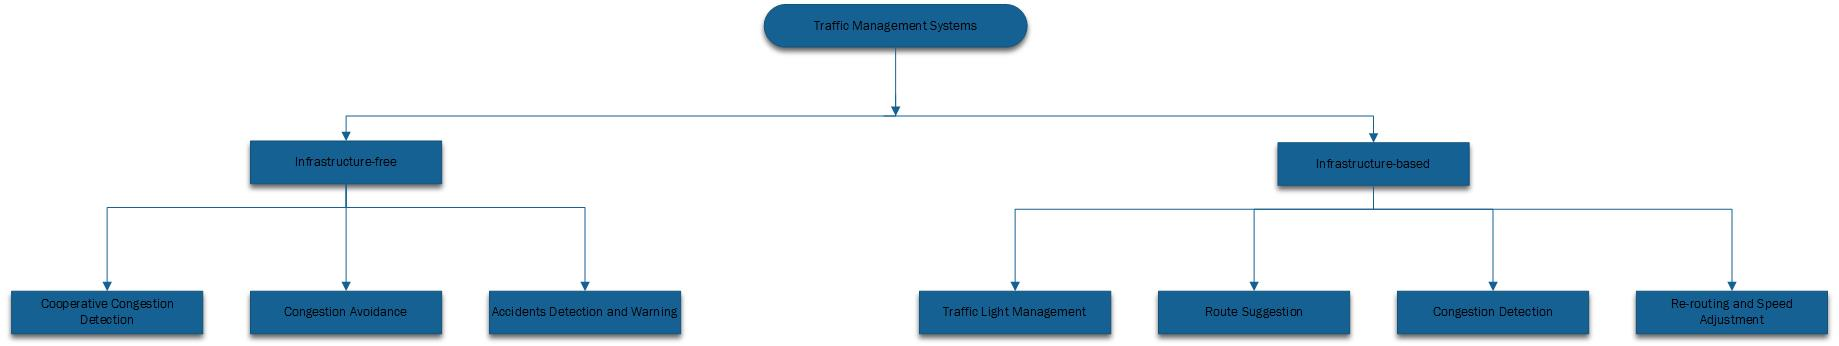
\includegraphics[width=7in]{flowDiagramTrafficManagement}
\caption{Traffic Management Systems Classification}
\label{flow_diagm}
\end{figure*}

by clocks or they utilize sensors snared to a concentrated framework. El-Tantawy's idea utilizes cameras and PCs in every individual crossing point to in a flash read traffic information every which way and change the length of the green light as needs be.
 Traffic congestion is by no means a new problem. In our personal view smart traffic management system is all about urban traffic systems, safety, pollution and energy consumption. TMS is all about real-time data gathering and using that data to manage the traffic congestion.But it can be argued, obviously, we as of now have conveyed "smart" advancements for traffic management, we have CCTV cameras to monitor activity. Obviously, the CCTV frameworks permit some kind of vehicle distinguishing proof and even vehicle numbering utilizing which we can gauge conceivable regions of traffic blockage in a city in light of which city directors endeavor to take essential activities. 
 
 Be that as it may, then even with the CCTV frameworks sent, congested driving conditions are extremely regular is most urban areas and towns crosswise over Canada in a startling occasion of a street mishap or a vehicle separate. In such a startling occasion, the whole TMS appears to separate prompting to terrible movement clog affecting versatility of vehicle and walkers. 
 
 Thus, it is not generally comprehending the reason and expected purpose the fundamental objectives of a smart traffic management arrangement needs accurate data to accomplish feasible portability, and securing exact and opportune information about explorers developments to search for a streamlining of the accessible means it should be a smart sensor based wireless system centered in light of gathering real-time data on traffic with segments for,vehicle counting,vehicle,identification,monitoring noise levels,CO (carbon monoxide) and tidy levels,gases concentrations,humidity, etc.Since it is wireless, there would be no compelling reason to uncovered streets, embrace development works and have street terminations as a component of its organization. Thus, the general cost of organization is much lower and in actuality a fast and speedy arrangement is conceivable.







\subsection{Organization of the Survey}
The rest of this survey shall be organized in the following manner. In the next section, a brief technical background of TMS will be provided. This will lead into the definition of various metrics which may be employed in order to characterize advanced traffic management architectures. Afterwards, the contribution of other surveys in this field will be detailed such as to clarify the novelty of this one. The latest research delving into TMS in internet of things (IoT) are presented in the following sections and are broken down into sub-classes as shown in Figure \ref{flow_diagm}. It is pointed out that these sub-classes have received general consensus from researchers and have been adopted from previous surveys in the field \cite{Botnet:Hoque,Zargar:DDOSFlood}. Finally, these findings will be interpreted and discussed so to draw insight into the future of TMS.

\section{Background}

Based on the VANET, vehicles require two types of communication resources. The first resource includes vehicle to vehicle (V2V) that deals in communicating with other vehicles using DSRC and the later one vehicle to infrastructure (V2I) using long distance communication resource i.e.  LTE. 

Vehicles on road receive data from road sensors, traffic lights and other networks employing OBU modules and forward it to the vehicles of its short range. However, they can also transmit data to RSU using V2I resources through access network. The access network is in turn connected to the cloud with core network and this is how the core networks forward the data to cloud, thus the TMS implementation being enhanced. The whole TMS process generally takes three stages to complete its service of detecting traffic congestion: (i) Data Collection, which involves in assembling data from multiple sources (ii) Data operation, which entirely depends on combining data collected from diverse sources and process it further to check if there is any error which may eventually deteriorate the safety of TMS and (iii) User end service, the service provided to user by means of different multimedia service systems.

\textit{Data Collection} is a module or sensor that keeps collecting traffic oriented data from different origins covering vehicles, roadside sensors, incorporated device sensor such as GPS. The module OBU assembled these data to be shared with TMC. The road sensor especially the module RSU have the records of data history of traffic including the information of traffic light, traffic condition of roads etc. Furthermore, the web resource gives accurate information on traffic data such as posting and sharing on various types of social media has merged the traffic scenerios and thus the traffic congestion being predicted.

\textit{Data Operation} enables traffic risk to be identified and estimated after executing the task of traffic information collection. For the TMS issue, it can be implemented both in infracstructure free and infrastructure-based system. In infrastructure-free system, vehicles share traffic risk information with other vehicles employing V2V technology which is distributed system. In the infrastructure-based, vehicles make proper use of main server such as TMC or other infrastructures in purpose of picking out the traffic risk information. It provides a better quality of  TMS service to people even if it has a long maintenance of greater amount of overhead compared to infrastructure free technology. 

\textit{User End Service} is provided to the user on account of identifying the traffic risk issues and avoiding the congestion. As per TMS theory, this service can be dispatched in both way infrastructure-free and infrastructure-based. Infrastructure free technology provides services including collision finding, collision avoiding which takes delay in response, whereas infrastructure-based technology offers better quality traffic management by providing the congestion identification, speed controlling and alternative way suggestion.

\subsection{Infrastructure-free TMS Taxonomy}
The pillars of Infrastructure-free TMS are as follows: 
\subsubsection{Cooperative congestion detection}
Enabling driver to react appropriately to changes in his immediate environment.
\subsubsection{Congestion avoidance}
V2V Communication  to streamline the operation of vehicles by overseeing vehicle movement, helping drivers with safety and sharing data, and in addition giving proper administrations to travellers.
\subsubsection{Accident detection and warning}
Occurrence cautioning projects are characterized as spacial projects, which build up a threat cautioning in reliance of the danger on the primary carriageway.

\noindent Table \ref{tab:V2Vmet} summarizes other V2V factors.

{
\tabulinesep=1mm
\begin{table}[!htb]
  \centering
  \begin{tabu} to 0.5\textwidth {|X[2,r]|X[6]|}
     \hline
      Collision warning&Cooperative forward collision warning, 
to be specific, to keep away from rear-end collisions.\cite{adHocNetworks:Hartenstein}\\\hline
      
      Wireless diagnosis &  Remote wireless diagnosis, in particular, to make the condition of the vehicle accessible for remote diagnosis\\\hline
      
     Signal synchronization & Traffic light ideal speed admonitory, to be specific, to help the driver to arrive during a green phase.\\\hline
     
     Efficacy and reliability & Where sender could misinterpret with falsely data to gain advantage. In this case a secured and authenticate network can secure the communication between vehicle in infrastructure-free TMS. \\\hline    
     Storage& We should note that in a system of vehicles, energy and storage space are adequately accessible. \\\hline
      
      
  \end{tabu}
  \smallskip
  \caption{Summary of Infrastructure-free or V2V factors}
  \label{tab:V2Vmet}
\end{table}
}

\subsection{Infrastructure-based TMS Taxonomy}
The four sub-categories of Infrastructure-based TMS are summarized below and are visualized in Figure \ref{flow_diagm}.

\subsubsection{Traffic light management}
To identify the nearness of traffic waiting up at the light.
\subsubsection{Route suggest}
At the point when a specific street portion presents indications of congestion, the service searches for adjacent vehicles to re-route.
\subsubsection{Congestion detection}
Traffic management here is to distinguish and control clog by utilizing a decision-making algorithm which decides how the traffic light works in view of the data gathered from smart devices.
\subsubsection{Rerouting and speed management}
TMS regulate road traffic by sequencing traffic movements and setting routes with the aim of ensuring smooth transportation behavior and limiting, as much as possible, transport delays.
\begin{figure}[!ht]
\centering
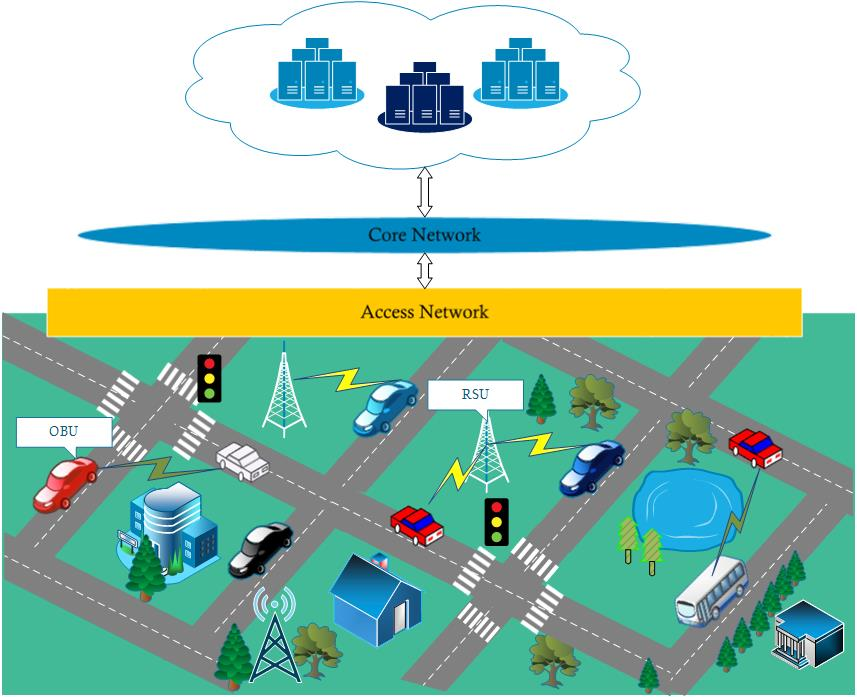
\includegraphics[width=3.5in]{wireless_traffice}
\caption{Over all TMS architecture}
\label{wireless}
\end{figure}



\section{Related Work}
Numerous surveys in the area of traffic management systems have been studied and considered a measurable extent for reducing the collision in roads, wait time of vehicles on traffic crossing points and emphasizing urgent vehicles. A \$423m project on Intelligent Transport System (ITS) was carried to improve Hong Kong's busiest road transport network RoadTraffic\footnote{http://www.roadtraffic-technology.com/projects/hong-kong/}. The project was not easy to implement on hilly terrains so as to take longer time from 2001 to 2010. The key element it performed to indentify congestion includes traffic data assembling, obseving, data processing and controlling congestion. This project has enabled an efficient traffic system in important highways, underpass roads and brach roads.

Sridhar \textit{et al.}\cite{gnawali2009collection} developed a pile of low cost sensor nodes due to its low maintenace requirement which is networked in wireless system and keeps role in keeping a pool of information of the vehicles running through the temporary work zones.

Al-Holou \textit{et al.} \cite{nellore2016survey} proposed a traffic management model in which vehicles greatly relies on traffic clog, sorrounding environment and traffic flow. His project deals with adaptive light controlling that minimize the traffic intensity and maximize the traffic flow using V2V/V2I technology. 

Christopher \textit{et al.}[4] implemented their project in University of Maryland focusing on the concept of high quality (HQ)digital video surveillance camera networked wirelessly. This project will enable efficient traffic analysis using better capturing HQ image and wireless network.

\section{Existing Infrastructure-free technology}
\subsection{Cooperative Congestion Detection}

Bauza \textit{et al.}\cite{bauza2013traffic} presented CoTEC(COperative Traffic congestion detECtion), a V2V communication based technology to identify traffic congestion assessed in large-scale broadway which accurately picks out and read the traffic congestion scenarios under different circumtances of traffic. Exchanging information through V2V or V2I communication, this technique enables road traffic information to be shared in a cooperative manner. Vehicles collaborately determine the surrounding traffic condition periodically broadcast by vehicles and CoTEC makes it possible by applying CAMs (Cooperative Awareness Messages) which is also considered as beacon messages. CoTEC maintains the fuzzy-logic based algorithm while detecting traffic congestion using beacon signals gained from other vehicles. CoTEC performs a traffic congestion quatization process based on the fuzzy logic mechanism to segment the congestion. Collecting the traffic data from different sources needs fuzzy logic that is based on Level Of Service (LOS) found in Highway Capacity Manual (HCM) \cite{araujo2014cartim}. LOS presents some operational statements while applying in the traffic flow. 

Araujo \textit{et al} \cite{milazzo1999quality} present CARTIM (Cooperative vehiculAR Traffic congestion Identifi-
cation and Minimization), a proposal which employ V2V connection on purpose of detecting traffic congestion. Their simulation work proved CARTIM efficiently detect congestion and minimize it. CARTIM collaboratively estimates the traffic congestion level which is the same task as CoTEC does and both systems have decision making with the implementation of fuzzy-logic mechanism. However, the fuzzy logic rules, both systems are implementing are different from others since both rules are built in different matrices presented on HCM. This is how they are unlike in fuzzy logic mechanism. Moreover, CARTIM proposes a heuristic decision to change the way, thus minimizing the traffic density while detecting congestion. 




\subsection{Congestion Avoidance}
Meneguette \textit{et al} \cite{meneguetteenhancing} develop UNCONDES (UrbanCONgestion Detection System) which involves in identifying traffic and reducing it in urban ares using V2V communication. Unlike the previous proposed model, UNCONDES is based on Artificial Neutral Network(ANN) to detect traffic congestion problem and it represents the dimension of traffic congestion, thus suggesting the  alternative route to avoid congestion. This is how this technology also decrease the amount of fuel consumption. ANN implemented in UNCONDES collects the data of speed and density of routes and it is done by receiving the beacons of all vehicles plying on the roads periodically \cite{yousefi2006vehicular}. The input parameter configured in ANN uses the data of vehicle speed and its density on roads and the congestion level of road used as output. ANN classifies the output into three levels of congestion \cite{meneguetteenhancing}. They are: 

Free: output is lower or equal to 0.3

Moderate: when the output is in between 0.3 and 0.7

Congested: Output is above or equal to 0.7


This is how a vehicle gets beacon messages from surrounding vehicles that contains data of classification level of congestion and based on that message it checks if it can pass the roads. If it finds congestion, then it follows the mechanism to avoid this route and get suggestion to take alternative pathway having less congestion.













\subsection{Accident Detection and Warning}
Souza \textit{et al.} \cite{de2016fully} proposed a fully distributed V2V communication based TMS, FASTER that develops the traffic efficiency by gathering the exact data of traffic for each vehicle. Based on this purpose, FASTER enables all vehicles acquire information of traffic scenarios and disseminate it to other neighbors. Therefore, the knowledge of traffic data is to be developed. To ease the execution, FASTER chunk  the whole scenarios in segments, named Districts on purpose of developing the knowledge of traffic in that particular division.  Moreover, roads under each district contain overall knowledge of road traffic density and speed of vehicles.  In this way, the district based information of traffic is shared with other vehicles through disseminating beacons. Due to the rapid changes of vehicle density and network architecture continual changes, VANET faces a limitation in employing data dissemination protocols, thus decreasing the dissemination capacity. This limitation is \textit{broadcast storm problem} \cite{souza2014add} that occurs especially when multiple vehicles plying on road try to transmit at the same time. FASTER has the ability to overcome this problem. Moreover, it has the mechanism to overcome the obstacles of \textit{resynchronizing effect} \cite{souza2014add} developed by IEEE 802.11p. After receiving all the knowledge of district, vehicles develop a graphical relation G=(V,E), [5] where V is a set of crossing points and E is a set of routes that represent the scenerio. Moreover, each road carries a weight focusing on the average speed of vehicles on road. Hence, FASTER allows each vehicles to have exact information of traffic condition.
Souza \textit{et al.} [8] propose a TMS based on inter-vehicle communication system which avoids the highly dense route and shorten the travel time, consequently lessen the fuel intake and spread of CO2 emission. To overcome the broadcast storm problem, this model implements DRIFT algorithm which increases the data disseminating capacity with low over head, thus disseminating the warning data of accident. 
Souza \textit{et al.} [9] propose a fully-distributed, pro-active TMS, GARUDA(Geographical
Accident aware to Reduce Urban Congestion) to reduce the congestion level in urban areas. GARUDA implements in three stages: (i) Information Generation (ii) Information Dissemination and (iii) Making Real Time Decision. \textit{Information Generation}: During mishap, the running vehicles share an alarm message with other forwarding vehicles to make them aware of the geographical coordinates of occurrence. In GARUDA, an OBD 2 system (On Board Diagnostic 2) is required to determine the real time information of vehicles, such as, speed and air bag status etc.Thus, GARUDA is able to detect the accident and pass this message to the next module. \textit{Information Dissemination}: During the disseminating stage, GEDDAI-NP (Geographical
Data Dissemination of Information and Alert Aware of Network
Partition) protocol is used to spread the message over network. Consequently, it circumvents the obstacles of broadcast storm problem, thus making short delay with low overhead and increasing the efficiency of disseminating capacity. \textit{Making Real Time Decision}: As soon as the alarm message being received, a decision of short delay is made using the \textit{Making Real Time Decision} module in application segment. Using this module, vehicles check if the accident location is suitable to pass. If not possible then a new route is suggested to avoid the accident place.








\begin{figure}[!ht]
\centering
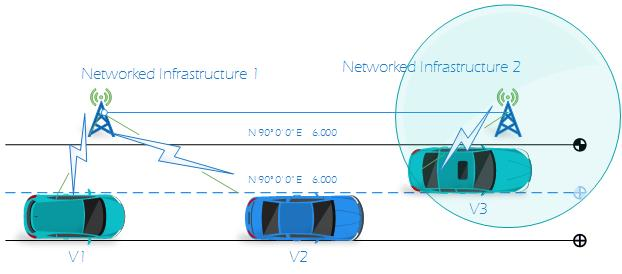
\includegraphics[width=3.5in]{V2I}
\caption{Vehicle to Infrastructure TMS}
\label{fig_ldosAttProf}
\end{figure}











\section{existing infrastructure-based technology}
\subsection{Traffic Light Management}
Rakha \textit{et al.} [10] come up with a V2I communication based model, a traffic light management system that is built in traffic crossing point for  intelligent Traffic Light (ITLs). It reduces the amount of time vehicles waste on traffic light intersection, thereby fuel is efficiently utilized which in turn limit the release of CO2. To  retain fuel  utilization in an  optimum level, each  vehicle  regulates  its  speed. Consequently, they don't have to wait long time on the traffic light intersection. 

\subsection{Route Suggestion}
Revisiting LDoS, two recent papers published by Wu \textit{et al.} \cite{Wu:LDoSMultifractal} and Bhuyan \textit{et al.} \cite{Bhuyan:partialRank} seek to provide a higher degree of detection, and ultimately mitigation, against such attacks. Both methods are deployed at the victim end and employ statistical methods to discriminate against attack traffic.

Wu \textit{et al.} present an analysis on the sensitivity of a statistical parameter, known as the singularity exponent, to LDoS attacks. The argument is that in a large scale, network traffic exhibits self-similarity while as a small-scale time series it is multifractal \cite{Wu:LDoSMultifractal}. The researchers look into the affect LDoS attack pulses have on the singularity exponent through a Multi fractal Detrended Fluctuation Analysis (MF-DFA) algorithm. Next, the researchers present their developed algorithm in the estimation of the singularity exponent based on network traffic. Through their experimentation, it was found that as traffic becomes busty, the singularity exponent decreases. In these tests, the ideal detection threshold was found as 0.6 --- offering a detection probability of 92\% along with a false positive and false negative rate of 9\% and 8\%, respectively \cite{Wu:LDoSMultifractal}.

Bhuyan \textit{et al.} estimates a parameter known as the correlation coefficient to determine the pairwise linear relationship of sampled network traffic. This value is bounded between [-1,1] signifying the amount of similarity --- with zero being none at all. They then calculate the partial rank correlation based on the already calculated correlation coefficient and this rank is compared to pre-defined thresholds. Two assumptions made in this work are that pairs of attack traffic have a rank of 1 and that attack and legitimate traffic follow Poisson and Gaussian distributions, respectively \cite{Bhuyan:partialRank}. That being said, the definition of such thresholds is highly dependent on an initial training phase containing both legitimate and attack traffic.

Although not particular to LDoS, the work of Tan \textit{et al.} also employs statistical correlation analysis to detect DoS attacks \cite{Tan:MCA}. Multivariate Correlation Analysis (MCA) is employed in order to address the issues of LDoS attacks that linearly change commonly monitored features to avoid detection as well as only being able to identify \textit{all} packets in a sample as either legitimate or not. This is accomplished by considering traffic samples individually. In addition, this method requires no historical traffic profiling to carry out analysis.

First, ingress traffic is monitored in order to build a network profile. Next, MCA is performed; Tan \textit{et al.} present an optimized algorithm employing a triangle area map scheme. This scheme identifies how the features of a sample series are geometrically correlated. Lastly, an anomaly based detection system is used in acting upon the features discovered by MCA. This system requires a 'normal profile' and a tolerance of deviation \cite{Tan:MCA}.

In benchmarking this solution, the researchers have put it up against six different DoS attacks. While the back, Smurf, and pod attacks were detected at rates in the high 90s (with a threshold of 3 standard deviations of the Mahalanobis Distances) whereas the teardrop and Neptune attacks were detected at a rate of about 50\%. The LAND attack was not detected at all. At the same threshold as above, the false positive rate was found to be 0.53\% \cite{Tan:MCA}. These deficiencies were addressed by Tan \textit{et al.} by use of data normalization which improved the detection rate of all the tested attacks at the cost of a larger false positive rate.  

Another form of victim end defense is an affirmation challenge which appears in the form of a puzzle. Such puzzles are intended to be easily generated by the server, reasonably difficult to solve for the client, and --- again --- easy for the server to check the answer's correctness. For instance, during a potential DoS attack originating form many different spoofed IP addresses; in this situation, the server will not expedite client requests or allocate memory until the correct solution is given. This mechanism can be prone to solution replay attacks by savvy clients.

With puzzles, there is no discrimination of legitimate traffic as all clients must bear the burden. This infrastructure is meant as a deterrent for attackers since establishing a connection to the content provider will waste their resources. For this reason, puzzles can be thought of as having a preventative action time. Also, it is noted by work in this area that dynamic puzzle difficulty based on the server's instantaneous workload has not been explored. Abliz \textit{et al.} introduce productive puzzles to address the issues of dynamism, solution replaying, and providing some utility out of the entire process. 

These so-called productive puzzles are a novel system for safeguarding against DDoS attacks \cite{Abliz:Puzz}. They intend to utilize undertakings from real applications and administrations rather than tedious cryptographic calculations for the sole purpose of posing a challenge to the client. With a generic puzzle generation framework, the output of the framework can be tailored to yield a solution relevant to a particular service. A Productive Puzzle Protocol (PPP) is presented by the authors to achieve these objectives. Moreover, a novel cache calculation is developed in consideration with the replay attack. Finally, Abliz \textit{et al.} assess the server's workload so that the difficulty is proportional. 

\subsection{Congestion Detection}
Miao \textit{et al.} present a real-time method for detecting Internet-wide SYN flooding attacks that can be deployed at network borders like Points of Presence (PoP) \cite{RealtimeDetection:Miao}. It works by first identifying eight attack scenarios based on whether the attacker is inside of a certain network $N$ or not (called the position of the attacker), the position of the victim and the position of the source IP address. Then, this method records metrics on SYN and SYN-ACK packet flow in five-minute intervals and, using an anomaly detection function on these metrics, builds a detection vector. Each attack scenario can then be mapped to a unique pair composed of the position of the victim and the detection vector using an algorithm the authors called WSAND.

This detection method has been implemented and used on 28 PoPs in the China Education and Research Network (CERNET) since the end of 2013. Attacks detected in March 2014, of which there were 207622, are discussed in the paper. The team behind this research manually validated part of those detection using (incomplete) IP traces and found that 92.5\% of them were correct, while the rest were either false positives or the IP traces didn't contain enough information for validation. The team plans on capturing complete packet traces to perform more thorough validation in the future.


\subsection{Re-routing and Speed Adjustment}



.



\section{Interpretation and Discussion of Findings}

It was found that the attack classifications adopted from \cite{Botnet:Hoque,Zargar:DDOSFlood} are still relevant in regards to recent findings. That is, no new research in the field constitutes a brand new category. This does not come as a surprise due to the maturity of studies in DoS. Furthermore, it was found that most advances in DoS stem from either oversights in protocol specifications or operating under the assumption that a design will not be misused or abused (as seen in \cite{DoSTCPAnalysis:Schuba,Li:LAAEM,OffPath:Cao}). Attacks based purely on bandwidth exhaustion, flooding, and even malforming packets are not as active.

In the case of defenses, a wealth of information was revealed by the literature review of this survey. It is noted that purely source end solutions have not been as recently active as other categories. Observations explaining this are compiled in Table \ref{tab:defense}. The surveyed mechanisms expand on, and optimize, existing techniques and others make use of paradigms with growing popularity. Examples of this are found in the use of the cloud environment to provide cost-effective DoS Elusion and SDN as with Bohatei. As these systems become increasingly sophisticated and distributed, they must consider practicality. Such is covered in Steinberger \textit{et al.}'s efforts to standardize a collaborative event-based messaging protocol.

%TODO



\section{Conclusions}
In this paper, we briefly discussed traffic management systems  before presenting a classification and taxonomy inspired by previous surveys in the field for both infrastructure-free and infrastructure-based mechanisms. We then introduced recent research papers on the subject of infrastructure-free targeting the V2V communications, followed by infrastructure-based techniques collaborating with V2I technique, all of which we classified and characterized following our taxonomy. Finally, we interpreted and discussed our findings.

Though infrastructure-based communication is a very mature field and research in the area is abundant, it is still in evolution and problems still remain unsolved. Infrastructure-free techniques are making great advances, becoming more and more effective and sophisticated as we have shown, but the effectiveness of even the most recent research such as the one traffic solution\footnote{http://dyn.com/blog/dyn-analysis-summary-of-friday-october-21-attack/} demonstrate that work still needs to be done in that regard.

\bibliographystyle{ieeetr}
\bibliography{papers.bib}
% use section* for acknowledgment
%\section*{Acknowledgment}
\end{document}